\documentclass[a4paper,oneside,10pt]{article}
% Alternative Options:
%	Paper Size: a4paper / a5paper / b5paper / letterpaper / legalpaper / executivepaper
% Duplex: oneside / twoside
% Base Font Size: 10pt / 11pt / 12pt

\usepackage[USenglish]{babel} %francais, polish, spanish, ...
\usepackage[T1]{fontenc}
\usepackage[ansinew]{inputenc}
\usepackage{lmodern} %Type1-font for non-english texts and characters
\usepackage{graphicx} %%For loading graphic files
\usepackage{amsmath}
\usepackage{amsthm}
\usepackage{amsfonts}

\begin{document}

\pagestyle{empty} %No headings for the first pages.



\title{FAST LANE TRACKING FOR AUTONOMOUS URBAN DRIVING USING HIDDEN MARKOV MODELS AND MULTIRESOLUTION HOUGH TRANSFORM}
\author{}

\maketitle

\begin{abstract}
Lane tracking is one of the most important processes for autonomous vehicles because the navigable region usually stands between the lanes, especially in urban environments. Hough transform is one of the most popular algorithms for lane detection. A robust lane tracking method is also required for reducing the effect of the noise and the required processing time. In this paper, we present a new lane tracking method which uses a partitioning technique for obtaining multi-resolution Hough Transform (MHT) of the acquired vision data. After the detection process, for tracking the detected lanes, a Hidden Markov Model (HMM) based method is proposed. 
\end{abstract}

\section{Introduction}

Although vehicle manufacturers deploy more intelligence in their newest models, the current applications are usually focused on driver assistance and early warning systems ~\cite{connolly09, piao08}. However, in the near future, intelligent vehicles will also enforce the traffic regulations. For example, speed limit and traffic light violations are going to be detected by cars.

In order to identify traffic violations some basic properties associated with roads must be detected. One of the main violations is due to lane departure. Lane detection has been studied in several works and Hough Transform ~\cite{hough62} is one of the most common techniques ~\cite{li04,yu97,mccall06}. However, there are many other techniques in the literature for lane detection. Pomerleau et al. ~\cite{pomerleau95} used neural networks in their ALVIN system. Dynamic programming is used for eliminating outliers from detected line segments by Kang et al. ~\cite{kang03}.  In addition, Wang et al. ~\cite{wang04} used B-splines in order to fit lane markings. Different techniques have also been proposed for tracking the detected lanes and modeling the road. Kalman filtering ~\cite{kreucher98} and particle filtering ~\cite{apostoloff03,zhou06} are the two most common  techniques used in lane tracking. A more detailed survey for lane detection strategies can be found on ~\cite{mccall06}. 

With this motivation, the aim of the ADES project is to develop a framework for evaluating the drivers against the traffic rules. The applications of the resulting system include but not limited to the following items;

\begin{itemize}
    \item Deter drivers from violating traffic rules
    \item Automation of driver license examinations
    \item Supervising the development of autonomous urban driving
\end{itemize}

\noindent The project consists of two major parts. The first part is acquiring the necessary information from various sensors whereas the second part is processing these knowledge to evaluate the driver's actions. 

In this work we present a new approach for obtaining lane boundaries from vision data. The proposed approach uses Multiresolution Hough Transform (MHT) for detecting lane markers followed by an HMM model for tracking them. 

The next section provides information about the road and lane types considered in the project. In  section ~\ref{sec:pa} the difference of the proposed Hough Transform from the classical one is given. The proposed technique for tracking the lanes are also discussed in this section. The following section explains the details of the experimental setup and present the results.

\section {Roads and Lane Types}

The scope of this work is detecting the lanes on main streets or motorways where there is at least three or more lanes, including shoulder lines and centerlines. One way roads, alleys and any other type of unstructured roads are beyond the scope of this work. In addition, the following road markings are considered
\begin{itemize}
    \item {\bf Single broken line:} Passing is allowed
    \item {\bf Single solid line:} Pass only to avoid a hazard
    \item {\bf Double solid line:} Passing is prohibited
\end{itemize}
\noindent where the colors of the markings are expected to be white or yellow. The application tries to locate at most three lines which is the maximum number of lines the vehicle can interact when leaving one lane and entering the other lane. And most of the time, the vehicle stands between one centerline and one shoulder line in main streets, or two centerlines in motorways.

\section{Proposed Approach}
\label{sec:pa}

The proposed approach employs MHT for lane detection, followed by two HMM models for radius and orientation of the candidate lanes.


\subsection{Multiresolution Hough Transform}

The classical Hough transformation approach processes the entire vision data in order to detect the lines. This scenario has two main drawbacks. First, the occluded lines (i.e. another car passing through the line) become noisy since the transformed relative intensity of the line decreases. Second, the relative intensity of the lines also decreases at the curves in the road. The proposed solution divides the road image into partitions, where the sizes of the partitions are inversely proportional to the distance of the partition to the vehicle. 

After the image is partitioned, several preprocessing steps are required before applying the Hough transform. These preprocessing steps should be fast because the Hough transform is already computationally expensive for real time applications. Since edge detection techniques are usually computationally expensive for real time applications ~\cite{canny86,ratnayake06}, each partition is converted to binary images via applying a threshold filter after a color remapping process. 

\begin{figure}
\begin{center}
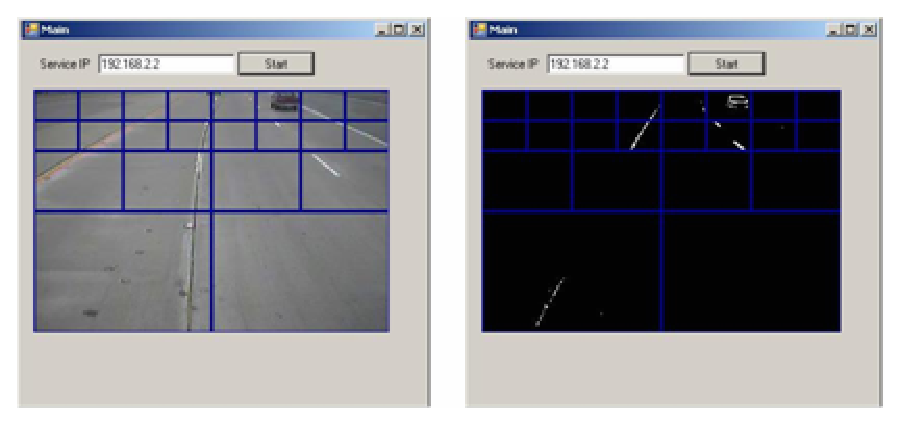
\includegraphics[scale=0.5]{fig1}
\end{center}
\caption{(a) Partitioned image, (b) Binary image.}
\label{aba:fig1}
\end{figure} 

After binaization process, a separate Hough transformation is applied to each single partition. The most intense line in each partition, which is the candidate line segment, is taken into consideration in order to find the global lanes in the image. Since the Hough lines are represented in polar coordinates \textit{(r, $\theta $)} instead of cartesian coordinates \textit{(x, y)}, the candidate lines are grouped according to their slopes and distances to the center of the image as well as their intensities. The center of the frame is chosen as the origin. 

\begin{figure}
\begin{center}
\includegraphics[scale=0.5]{fig2}
\end{center}
\caption{(a) Candidate lines, (b) Transformed line, (c) Detected lines.}
\label{aba:fig2}
\end{figure} 

The transformation of the lines basically changes the origin of the polar coordinates for each transformed line which is achieved by the following translation,

\begin{equation} \label{GrindEQ__1_} 
\begin{array}{l} {r'\, \, =\, r+(x-x')\cos (\theta )+(y-y')\sin (\theta )} \\ {\theta '=\, \theta } \end{array} 
\end{equation} 


\noindent where \textit{(r', $\theta $')} is the polar coordinates of the transformed Hough line \textit{(r, $\theta $)}. Note that the translation of the center of the Hough transformation is from \textit{(x, y)} to \textit{(x', y')}. 

After the lines are grouped, the most intense three clusters are assigned as the lanes. However, there may be less than three lanes if the sum of the intensities of the candidate lines is less than a threshold value.


\subsection{Lane Tracking}

For lane tracking, HMM is used to represent the relation between the current frame and its successor ~\cite{rabiner86}. Each line in a specific frame is represented by an individual \textit{(r, $\theta $)} pair. In the succeeding frame, the process will most probably observe the same line at \textit{(r', $\theta $')} which is not very far from the position of the line in the previous frame. The probability of observing \textit{(r', $\theta $')} pair in the next frame is modeled as an HMM problem. In addition, \textit{$\theta $} and $r$ values are modeled by two different HMM. The \textit{$\theta $} value is discretized as (0, 1, 2, 3\dots 178, 179) where the \textit{r} value is discretized at the pixel level. This discretization schema is used in both transmission and emission matrices. The emission probability matrix shows the probability of observing \textit{$\theta $'} (or \textit{r'}) in the next frame, having observed \textit{$\theta $} (or \textit{r}) in the current frame. In our implementation, the observation and state transition matrix values are derived from two Gaussian distributions with different deviations. The deviation of the transition matrix is assigned a smaller value than the observation matrix, which means, the state transition matrix aims to preserve the current state whereas the observation matrix promotes the exploration behavior.

\section{Experiment}

The proposed approach is implemented and tested on a relatively short video sequence of an urban drive. In addition, the new approach is compared with the classical Hough transform where the entire image is processed and the most intense lines are accepted as candidate lines. The properties of the video are given in \ref{aba:table1}.

\begin{table}
\caption{Properties of video sequence.}
\centering
% Table generated by Excel2LaTeX from sheet 'tables'
{\footnotesize
\begin{tabular}{|l|r|}
\hline
{\bf Camera Position:} & Front console of the car. \\
\hline
{\bf Resolution:} & 512x288 \\
\hline
{\bf Frame Rate:} & 29.97 \\
\hline
{\bf Length:} & 34 sec. \\
\hline
\end{tabular}  
}
\label{aba:table1}
\end{table}

\subsection{Setup}

As the first step of the experiment, the image is converted to a binary image by using color remapping. The mapping for each pixel from 24bit RGB value to binary value is given in Table 2.

\begin{table}
\caption{Color remapping.}
\centering
{\footnotesize
% Table generated by Excel2LaTeX from sheet 'tables'
\begin{tabular}{|r|r|r|r|}
\hline
{\bf Pixel Value} & {\bf Red} & {\bf Green} & {\bf Blue} \\
\hline
{\bf 0-176} & 0 & 0 & 0 \\
\hline
{\bf 176-196} & 1 & 1 & 0 \\
\hline
{\bf 196-255} & 1 & 1 & 1 \\
\hline
\end{tabular}  
}  
\label{aba:table2}
\end{table}

\noindent This binarization favors the white and yellow parts of the images. The values are manually crafted for the video sample. More discussions about improving the color remapping can be found in the next section.

The next step is to determine the partitions of the image on which the Hough transforms will be applied. Although the image is 288 pixels high, only the bottommost 116 pixels are used since the road remains in this lower part of the image. The accuracy of this assumption may slightly differ depending on the slope.

\begin{figure}
\begin{center}
\includegraphics[scale=0.5]{fig3}
\end{center}
\caption{Image partitions.}
\label{aba:fig3}
\end{figure} 

The widths of the partitions are 32, 64, and 128 pixels from top to bottom. And the heights are 32, 42, and 42 pixels respectively as shown in Figure 3. These values are assigned according to the position of the camera. After the partitions are calculated, Hough transformation is applied to each partition as described in the previous section.  The most promising three lines are assigned as the candidate lane markers. But there may be less than three lines if the intensity of the calculated lines are less than an empirically assigned threshold. The experiment shows that the proposed approach usually detects only two lines most of the time.

After finding the lane markers, HMM method is used to track the lanes. The values of the emission and transition matrices are derived using Gaussian assumption. The deviation of the transition matrix is assigned as 1 and the deviation of the emission matrix is taken as 2. Two separate models are prepared for the \textit{$\theta $} and \textit{r} values of the candidate lane markers. The transition and emission matrices are given in Tables 3 and 4. Since the \textit{$\theta $} values 0 and 179 are actually very close, the emission and transmission values are the same for 1 and 179 in \textit{$\theta $} matrices. In addition, the range of the \textit{r} matrices is (0, 282) because the maximum possible distance for any detected line is 282 pixels where the height of the processed part of the image is 116 and width of the image is 512.

\begin{table}
\caption{(a) Transmission matrix for \textit{r}, (b) Transmission matrix for \textit{$\theta $}.}
\centering
{\scriptsize
\begin{tabular}{|r|r|r|r|r|r|r|r|r|r|}
\hline
{\bf {\normalsize $r$}} & {\bf 0} & {\bf 1} & {\bf 2} & {\bf 3} & ... & {\bf 279} & {\bf 280} & {\bf 281} & {\bf 282} \\
\hline
{\bf 0} & 0,3989 & 0,2420 & 0,0540 & 0,0044 & ... & 0,0000 & 0,0000 & 0,0000 & 0,0000 \\
\hline
{\bf 1} & 0,2420 & 0,3989 & 0,2420 & 0,0540 & ... & 0,0000 & 0,0000 & 0,0000 & 0,0000 \\
\hline
{\bf 2} & 0,0540 & 0,2420 & 0,3989 & 0,2420 & ... & 0,0000 & 0,0000 & 0,0000 & 0,0000 \\
\hline
... & ... & ... & ... & ... & ... & ... & ... & ... & ... \\
\hline
{\bf 280} & 0,0000 & 0,0000 & 0,0000 & 0,0000 & ... & 0,2420 & 0,3989 & 0,2420 & 0,0540 \\
\hline
{\bf 281} & 0,0000 & 0,0000 & 0,0000 & 0,0000 & ... & 0,0540 & 0,2420 & 0,3989 & 0,2420 \\
\hline
{\bf 282} & 0,0000 & 0,0000 & 0,0000 & 0,0000 & ... & 0,0044 & 0,0540 & 0,2420 & 0,3989 \\
\hline
\multicolumn{10}{c}{} \\
\hline
{\bf {\normalsize $\theta$}} & {\bf 0} & {\bf 1} & {\bf 2} & {\bf 3} & ... & {\bf 176} & {\bf 177} & {\bf 178} & {\bf 179} \\
\hline
{\bf 0} & 0,3989 & 0,2420 & 0,0540 & 0,0044 & ... & 0,0001 & 0,0044 & 0,0540 & 0,2420 \\
\hline
{\bf 1} & 0,2420 & 0,3989 & 0,2420 & 0,0540 & ... & 0,0000 & 0,0001 & 0,0044 & 0,0540 \\
\hline
{\bf 2} & 0,0540 & 0,2420 & 0,3989 & 0,2420 & ... & 0,0000 & 0,0000 & 0,0001 & 0,0044 \\
\hline
... & ... & ... & ... & ... & ... & ... & ... & ... & ... \\
\hline
{\bf 177} & 0,0044 & 0,0001 & 0,0000 & 0,0000 & ... & 0,2420 & 0,3989 & 0,2420 & 0,0540 \\
\hline
{\bf 178} & 0,0540 & 0,0044 & 0,0001 & 0,0000 & ... & 0,0540 & 0,2420 & 0,3989 & 0,2420 \\
\hline
{\bf 179} & 0,2420 & 0,0540 & 0,0044 & 0,0001 & ... & 0,0044 & 0,0540 & 0,2420 & 0,3989 \\
\hline
\end{tabular}  
}
\label{aba:table3}
\end{table}

\begin{table}
\caption{(a) Emission matrix for \textit{r}, (b) Emission matrix for \textit{$\theta $}.}
\centering
{\scriptsize
\begin{tabular}{|r|r|r|r|r|r|r|r|r|r|}
\hline
{\bf {\normalsize $r$}} & {\bf 0} & {\bf 1} & {\bf 2} & {\bf 3} & {\bf 4} & {\bf 5} & {\bf ...} & {\bf 281} & {\bf 282} \\
\hline
{\bf 0} & 0,1995 & 0,1760 & 0,1210 & 0,0648 & 0,0270 & 0,0088 & ... & 0,0000 & 0,0000 \\
\hline
{\bf 1} & 0,1760 & 0,1995 & 0,1760 & 0,1210 & 0,0648 & 0,0270 & ... & 0,0000 & 0,0000 \\
\hline
{\bf 2} & 0,1210 & 0,1760 & 0,1995 & 0,1760 & 0,1210 & 0,0648 & ... & 0,0000 & 0,0000 \\
\hline
{\bf 3} & 0,0648 & 0,1210 & 0,1760 & 0,1995 & 0,1760 & 0,1210 & ... & 0,0000 & 0,0000 \\
\hline
{\bf 4} & 0,0270 & 0,0648 & 0,1210 & 0,1760 & 0,1995 & 0,1760 & ... & 0,0000 & 0,0000 \\
\hline
... & ... & ... & ... & ... & ... & ... & ... & ... & ... \\
\hline
{\bf 281} & 0,0000 & 0,0000 & 0,0000 & 0,0000 & 0,0000 & 0,0000 & ... & 0,1995 & 0,1760 \\
\hline
{\bf 282} & 0,0000 & 0,0000 & 0,0000 & 0,0000 & 0,0000 & 0,0000 & ... & 0,1760 & 0,1995 \\
\hline
\multicolumn{10}{c}{} \\
\hline
{\bf {\normalsize $\theta$}} & {\bf 0} & {\bf 1} & {\bf 2} & {\bf 3} & {\bf 4} & {\bf 5} & {\bf ...} & {\bf 178} & {\bf 179} \\
\hline
{\bf 0} & 0,1995 & 0,1760 & 0,1210 & 0,0648 & 0,0270 & 0,0088 & ... & 0,1210 & 0,1760 \\
\hline
{\bf 1} & 0,1760 & 0,1995 & 0,1760 & 0,1210 & 0,0648 & 0,0270 & ... & 0,0648 & 0,1210 \\
\hline
{\bf 2} & 0,1210 & 0,1760 & 0,1995 & 0,1760 & 0,1210 & 0,0648 & ... & 0,0270 & 0,0648 \\
\hline
{\bf 3} & 0,0648 & 0,1210 & 0,1760 & 0,1995 & 0,1760 & 0,1210 & ... & 0,0088 & 0,0270 \\
\hline
{\bf 4} & 0,0270 & 0,0648 & 0,1210 & 0,1760 & 0,1995 & 0,1760 & ... & 0,0022 & 0,0088 \\
\hline
... & ... & ... & ... & ... & ... & ... & ... & ... & ... \\
\hline
{\bf 178} & 0,1210 & 0,0648 & 0,0270 & 0,0088 & 0,0022 & 0,0004 & ... & 0,1995 & 0,1760 \\
\hline
{\bf 179} & 0,1760 & 0,1210 & 0,0648 & 0,0270 & 0,0088 & 0,0022 & ... & 0,1760 & 0,1995 \\
\hline
\end{tabular} 
} 
\label{aba:table4}
\end{table}

\subsection{Results}

The proposed approach managed to detect and track at least one line in most of the sequence. In addition, false positives are reduced to an acceptable level. In order to validate the results, the proposed approach is compared with the classical Hough Transform approach. In this method, the same part of the image is processed using the Hough transform routine. The most intensive 10 lines are merged according to their \textit{r }and \textit{$\theta $} values. Finally three or less candidate lines are selected as the lane markers. 

The major differences between the two approaches are shown in Figure 4. The images on the left hand side are the detected or missed lines by the classical approach. The right hand side images are the outputs of the new approach for the same frames which show that the new approach is more robust and accurate.

The computational cost of the proposed approach can be compared as follows. The average processing time is 21.25 milliseconds for a laptop PC with Intel T2050 processor at 1.6 GHz whereas the average cost of the classical approach is 15.29 milliseconds. 

The results of the experiments for both the proposed approach and the classical method are presented in sample video files which can be found in the project website ~\cite{ades09}.

\section{Conclusions}

Lane tracking is one of the major tasks in autonomous urban driving. A hybrid solution of MHT with HMM is applied in this work, and the performance of the system is increased. However there are certain assumptions and shortcomings of the proposed approach. First of all, variable lightning and road conditions require adaptive color remapping. Although this is beyond the scope of this work, it is crucial for a final product. In addition, the proposed approach models the lane boundaries as lines, therefore an approximation is inevitable at curves. However, it is also possible to use combination of line segments which are detected at each image partition. As another future work, the emission matrix can be updated on the fly by already made decisions.

\begin{figure}
\begin{center}
\includegraphics[scale=0.5]{fig4}
\end{center}
\caption{Differences between classical Hough transformation and proposed approach.}
\label{aba:fig4}
\end{figure}

\section{Acknowledgements}
This work is a part of the ADES (Automatic Driver Evaluation System) Project in Artificial Intelligence Laboratory of Bo{\u g}azi{\c c}i University ~\cite{ades09}.

\bibliographystyle{unsrt}
\bibliography{LaneTracking}	

\end{document}

